This section provides analytical and numerical analysis of the density encoding in the Hermite basis. More specifically, we provide the choice of optimal model parameters and assess the quality of encoding. 

\subsection{Choice of parameters of the method}
Orthogonal Hermite functions (\ref{eq:hermiteFunction}) decay exponentially
after a certain distance and thus can encode information only within
some interval. We can estimate this interval using the formula for
the last root of a Hermite polynomial, $\xi_{1,N} \approx \frac{\sqrt{1+2N}}{\lambda}$
\cite{Math1995}, which gives an approximation for the half-size
of the bounding box that we can successfully encode:
%
\begin{equation}
L_{box}/2 \lesssim \frac{\sqrt{1+2N}}{\lambda}
\label{eq:encodingRegion}
\end{equation}
On the other hand, orthogonal Hermite functions are the eigenfunctions of the continuous Fourier transform (Eq. \ref{Eq:HermiteFourierImage}).
Therefore, Hermite decomposition of order $N$ can encode only a certain interval of frequencies.
Using the same approximation as in the case of the real-space interval, we obtain the following equation for the maximum encoding frequency:
\begin{equation}
\omega_{max}=\frac{\lambda}{2\pi}\sqrt{2N+1} \label{eq:OmegaMax}
\end{equation}
%
In case of the the Fourier series expansion on an interval $(0, L_{box})$, we can
use the same estimation for the maximum encoding index $M_{max}$ by setting $M_{max}=2L_{box} \omega_{max}$.
%
Resolution $R$  of an X-Ray electron density map is defined by the size of the reciprocal lattice as $R=1/(2\omega_{max})$, or, equivalently,  $R=L_{box} /M_{max}$.
Therefore, using resolution of the map $R$ and the order of the Fourier series expansion $M$, we can estimate the lower bound on the Hermite scaling parameter $\lambda$ required to encode all the reflexes of the electron density diffraction pattern to be
\begin{equation}
\lambda\gtrsim\frac{\pi}{\max(R,L_{box}/M)\sqrt{2N+1}} \label{eq:levelOfDetails}
\end{equation}
%
Here, we bounded the actual resolution by $L_{box}/M$, because this will be the limit allowed by the finite Fourier series of order $M$. 

The two inequalities (\ref{eq:encodingRegion}  and \ref{eq:levelOfDetails})
give approximate bounds on the scaling parameter $\lambda$,
provided that we know the size of the box $L_{box}$ containing a protein density and the resolution of the map $R$. 
Using these inequalities, we obtain the following relationship between parameters $\lambda$ and $N$:
%
\begin{equation}
\frac{\pi}{\sqrt{2N+1}\max(R,L_{box}/M)}\lesssim\lambda\lesssim2\frac{\sqrt{1+2N}}{L_{box}}\label{eq:relationLabmdaN}
,
\end{equation}
which is valid for sufficiently large values of $N$. 
%\blue{[The left bound defines the encoding square of the T-matrix. The right bound defines the amount of noise in the encoding square.]}
%
Nonetheless, we can use the following empirical estimation for the optimal value of $\lambda$ at any $N$:
\begin{equation}
\lambda_{opt} \approx \frac{\pi}{2\max(R,L_{box}/M)\sqrt{2N+1}}+\frac{\sqrt{1+2N}}{L_{box}}\label{eq:LambdaEstimate}
\end{equation}
%
Using dimensionless relative parameters $\lambda L_{box}$ and $L_{box}/R$ we may rewrite the previous expression as
\begin{equation}
\lambda L_{box} \approx \frac{\pi \min(L_{box}/R,M)}{2\sqrt{2N+1}}+\sqrt{1+2N}\label{RelativeEstimate}
\end{equation}
%
If at a given expansion order N there is no such parameter $\lambda$ that satisfies inequality  (\ref{eq:relationLabmdaN}), then 
the protein representation might involve information loss. Therefore, we can estimate the minimum
order $N_{min}$ of the Hermite expansion that allows this inequality to have solutions to be
\begin{equation}
N_{min} \approx \frac{\pi }{4} \min \left(\frac{L_{box}}{R} , M\right)
\label{eq:Nmin}
\end{equation}
Validity of the provided estimates and the graphical representation of the real--space and the reciprocal--space bounds on parameter $\lambda$
will be demonstrated in the following sections.


The maximum order of the Fourier expansion $M_{max}$ can be estimated from the resolution and the size of the density map as  $R=L_{box} /M_{max}$.
However, when finding the global maximum of the cross-correlation function, we need to sample the space of possible translations of a protein with respect to the EDM with a step several times finer than the EDM resolution $R$.
%
In protein crystallography, it is the common practice to set the 
sampling step size to $R/3$ \cite{afonine2003fast}. 
In principle, we can use the same reasoning in choosing the optimal number of rotations $N_{rot}$. 
%For example, 
When using spherical harmonics, the angular search step usually equals to the resolution of the basis, $2\pi/N$ \cite{garzon2007adp_em}.
In case of the Hermite basis, we propose to use the same criterion.



\subsection{The transfer matrix}
Below we describe an analytical model of encoding by the Hermite basis for the one-dimensional case.
Suppose we have a function  $f(x)$ that describes an electron density of a non-periodic object. 
Without loss of generality, we assume that this function is defined on a 1D interval of $(-L_{box}/2;+L_{box}/2)$.
This function has the following decomposition into Fourier series:
\begin{equation}
\tilde{f}^{exact}_{k} = \frac{1}{L_{box}}\int_{-L_{box}/2}^{+L_{box}/2} f(x)e^{-2\pi i k x/L_{box}}~dx
\end{equation}
We will refer to Fourier coefficients obtained using this expression as {\em exact}. 
%
The original function is then recovered by the inverse Fourier transform:
\begin{equation}
f(x) = \sum_{k=-\infty}^{+\infty} \tilde{f}^{exact}_{k}e^{2\pi i k x/L_{box}}
\end{equation}
%
On the other hand, our algorithm computes {\em approximate} Fourier coefficients using the Hermite to Fourier transform:
\begin{equation}
 \tilde{f}^{approx}_k=\frac{1}{L_{box}}\sum_{n=0}^{N}\hat{f}_{n}\tilde{\psi}_{n}(\frac{k}{L_{box}}; \lambda)
 \end{equation}
 %
Assuming that function $f(x)$ is zero outside of the bounding interval, Hermite coefficients $\hat{f}_{n}$ can be written as the finite integral:
%by assuming that the function is zero outside of the box:
\begin{equation}
\hat{f}_{n} = \int_{-L_{box}/2}^{+L_{box}/2} f(x) \psi_{n}(x; \lambda)~dx
\end{equation}
%
Now, we can express the {\em approximate} Fourier coefficients as a linear combination of the {\em exact} ones:
\begin{equation}
\tilde{f}^{approx}_{k} = \sum_{l=-\infty}^{+\infty} T_{k,l} \tilde{f}^{exact}_{l}, 
\label{Eq:fourierApproximation}
\end{equation}
where the  {\em transfer matrix} $T_{k,l}$ reads as:
\begin{equation}
T_{k,l} = \frac{1}{L_{box}}\sum_{n=0}^{N}  \tilde{\psi}_{n}(k; \lambda) \int_{-L_{box}/2}^{+L_{box}/2} \psi_{n}(x; \lambda) e^{2\pi i l x/L_{box}} dx~
\label{eq:Tmatrix}
\end{equation}
%
The transfer matrix acts as a linear filter in the reciprocal space and demonstrates how the input function is distorted by the finite size $N$ of the Hermite basis. 
We should note that, generally, its values are complex numbers.
%
This matrix can also be seen as a product of two matrices,
\begin{equation}
\bf T = \bf F^{(1)} \bf F^{(2)},
\label{eq:TmatrixProduct}
\end{equation}
where the first matrix is a scaled Fourier transform of the basis functions,
\begin{equation}
 F^{(1)}_{kn} =  \tilde{\psi}_{n}(k; \lambda) / \sqrt{L_{box}}
\label{eq:F1matrix}
\end{equation}
and the second matrix is  a scaled Fourier series of the basis functions,
\begin{equation}
F^{(2)}_{nl} = \int_{-L_{box}/2}^{+L_{box}/2} \psi_{n}(x; \lambda) e^{2\pi i l x/L_{box}} dx / \sqrt{L_{box}}
\label{eq:F2matrix}
\end{equation}
%
Figure \ref{fig:HermiteFDec} shows the absolute values of matrices $ \bf F^{(1)} $ and $\bf F^{(2)}$ computed with $\lambda=0.55$ and $L_{box}=23$ \AA. 
%
The values of the  Fourier series  $\bf F^{(2)}$ were computed numerically using adaptive  quadrature.
%
The dashed blue line shows the maximum encoding frequency $\omega_{max}$, according to Eq. \ref{eq:OmegaMax}, and bounds the encoding region. 
The solid black line on the right plot demonstrates the maximum order of the Hermite expansion (Eq. \ref{eq:encodingRegion}), after which the 
Fourier series encode mainly the frequencies near $\omega_{max}$.  This is because on a finite interval $(-L_{box}/2 ,+L_{box}/2)$, 
high-order Hermite basis functions become orthogonal to low-order Fourier basis functions. 
%

\begin{figure}[H]
\label{fig:HermiteFDec}
\begin{centering}
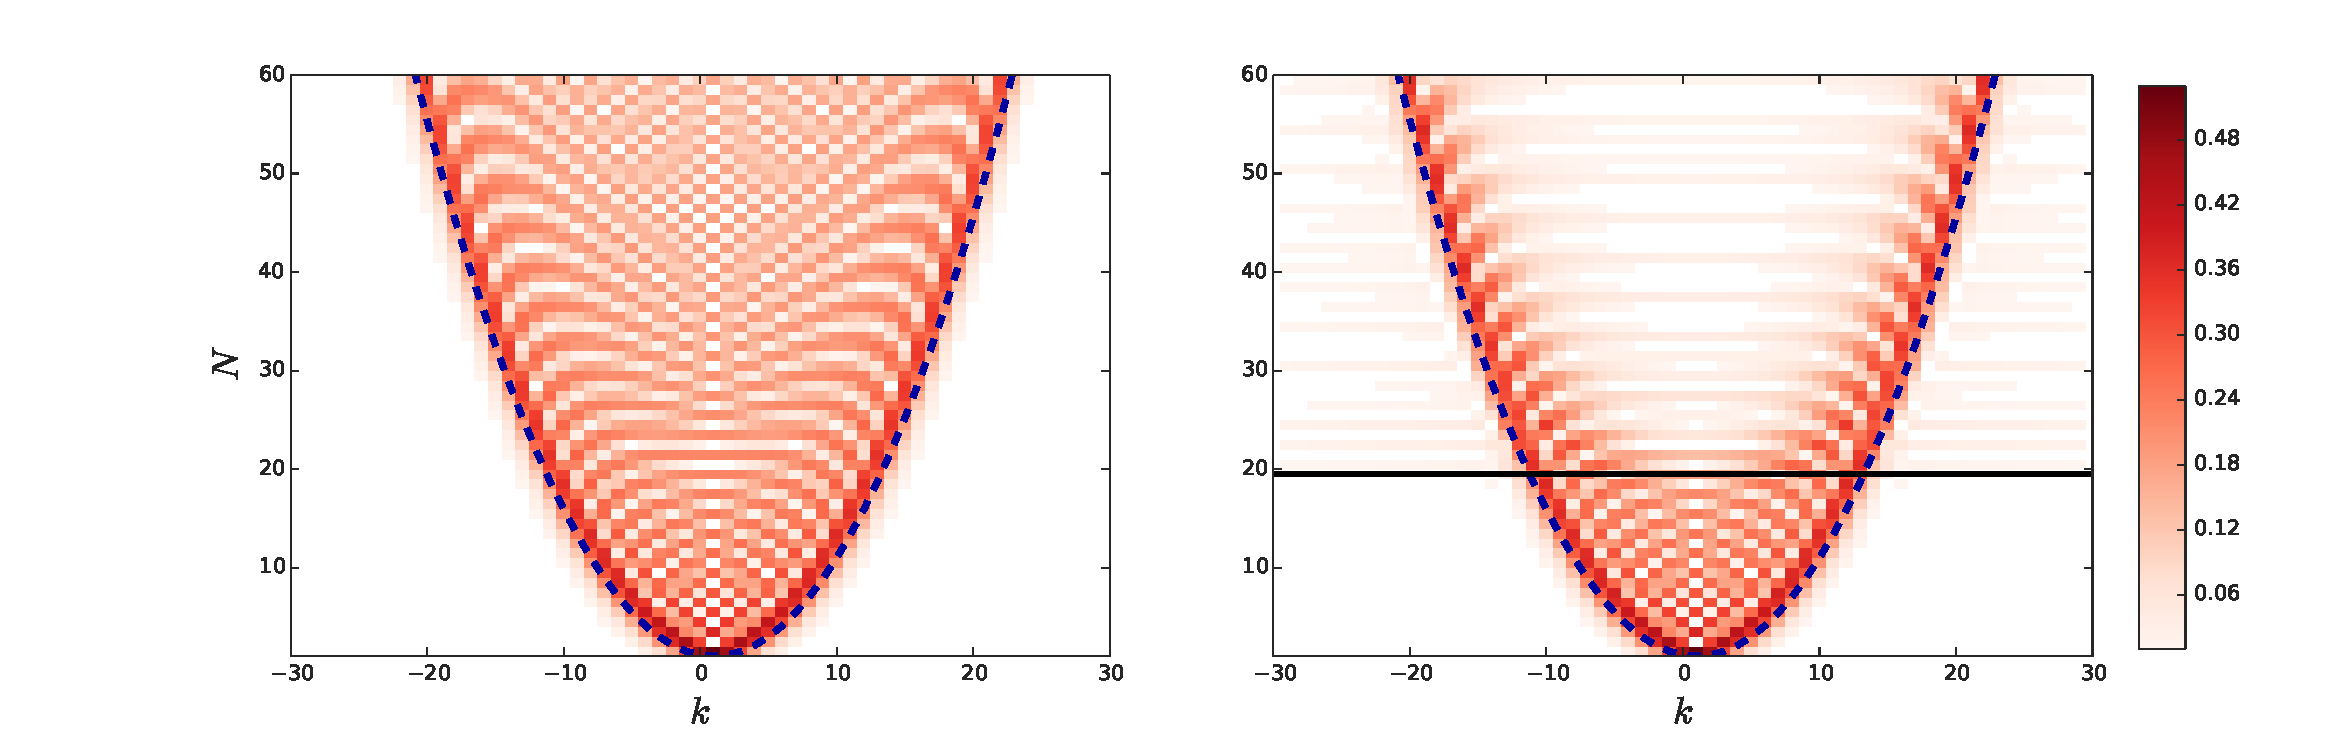
\includegraphics[width=\textwidth]{Hermite/Fig/HermiteFTransformAndSeries.pdf}
\par\end{centering}
\caption[Matrices $\bf{F^{(1)}}$ and $\bf{F^{(2)}}$]{
Absolute values of two matrices $\bf{F^{(1)}}$ and $\bf{F^{(2)}}$ that give the transfer matrix as their product (Eq. \ref{eq:TmatrixProduct}). These matrices are computed with the scaling parameter $\lambda=0.55$ and the input box size of $L_{box}=23.0$ \AA, which mimics
the first fitting example shown below.
Left: $\bf{F^{(1)}}$, the scaled Fourier transform of a 1D Hermite function as given by Eq. \ref{eq:F1matrix}. 
Right: $\bf{F^{(2)}}$, the scaled Fourier series of a 1D Hermite function as given by Eq. \ref{eq:F2matrix}.
The dashed blue line highlights the maximum encoded frequency according to Eq. \ref{eq:OmegaMax}.
The solid black line on the right plot shows the maximum Hermite decomposition order  $N_{max}$, at which the two matrices are still identical (Eq. \ref{eq:encodingRegion}).
}
\end{figure}


Figure \ref{fig:TmatrixesVsLambda} shows several examples of the absolute values of the transfer matrix components for three different values of the Hermite scaling parameter $\lambda$ and three values of the Hermite decomposition order
$N$.
The size of the transfer matrix was limited to $60\times 60$ and the box size $L_{box}$ was set to 23 \AA. 
The ideal transfer matrix should be identity, which is the case only at $N\rightarrow\infty$, as we demonstrate below.
We see, however, that the transfer matrix at small values of $\lambda$ encodes only low-order reflexes. 
The index of the last encoded reflex can be estimated from Eq. \ref{eq:OmegaMax} as $k_{max}=\sqrt{2N+1}\lambda L_{box}/(2\pi)$.
With the increase in  order $N$ and  parameter $\lambda$, the number of encoded frequencies  rises. 
At the same time, 
increasing the scaling parameter $\lambda$ makes the quality of encoding of all the frequencies worse, as we see in the right column. 
Therefore, it is very important to tune the value of $\lambda$ according to the class of input functions, such that the quality of encoding becomes optimal.
Below we will assess encoding quality by means of the  crystallographic R-factor.

\begin{figure}[H]
\label{fig:TmatrixesVsLambda}
\begin{centering}
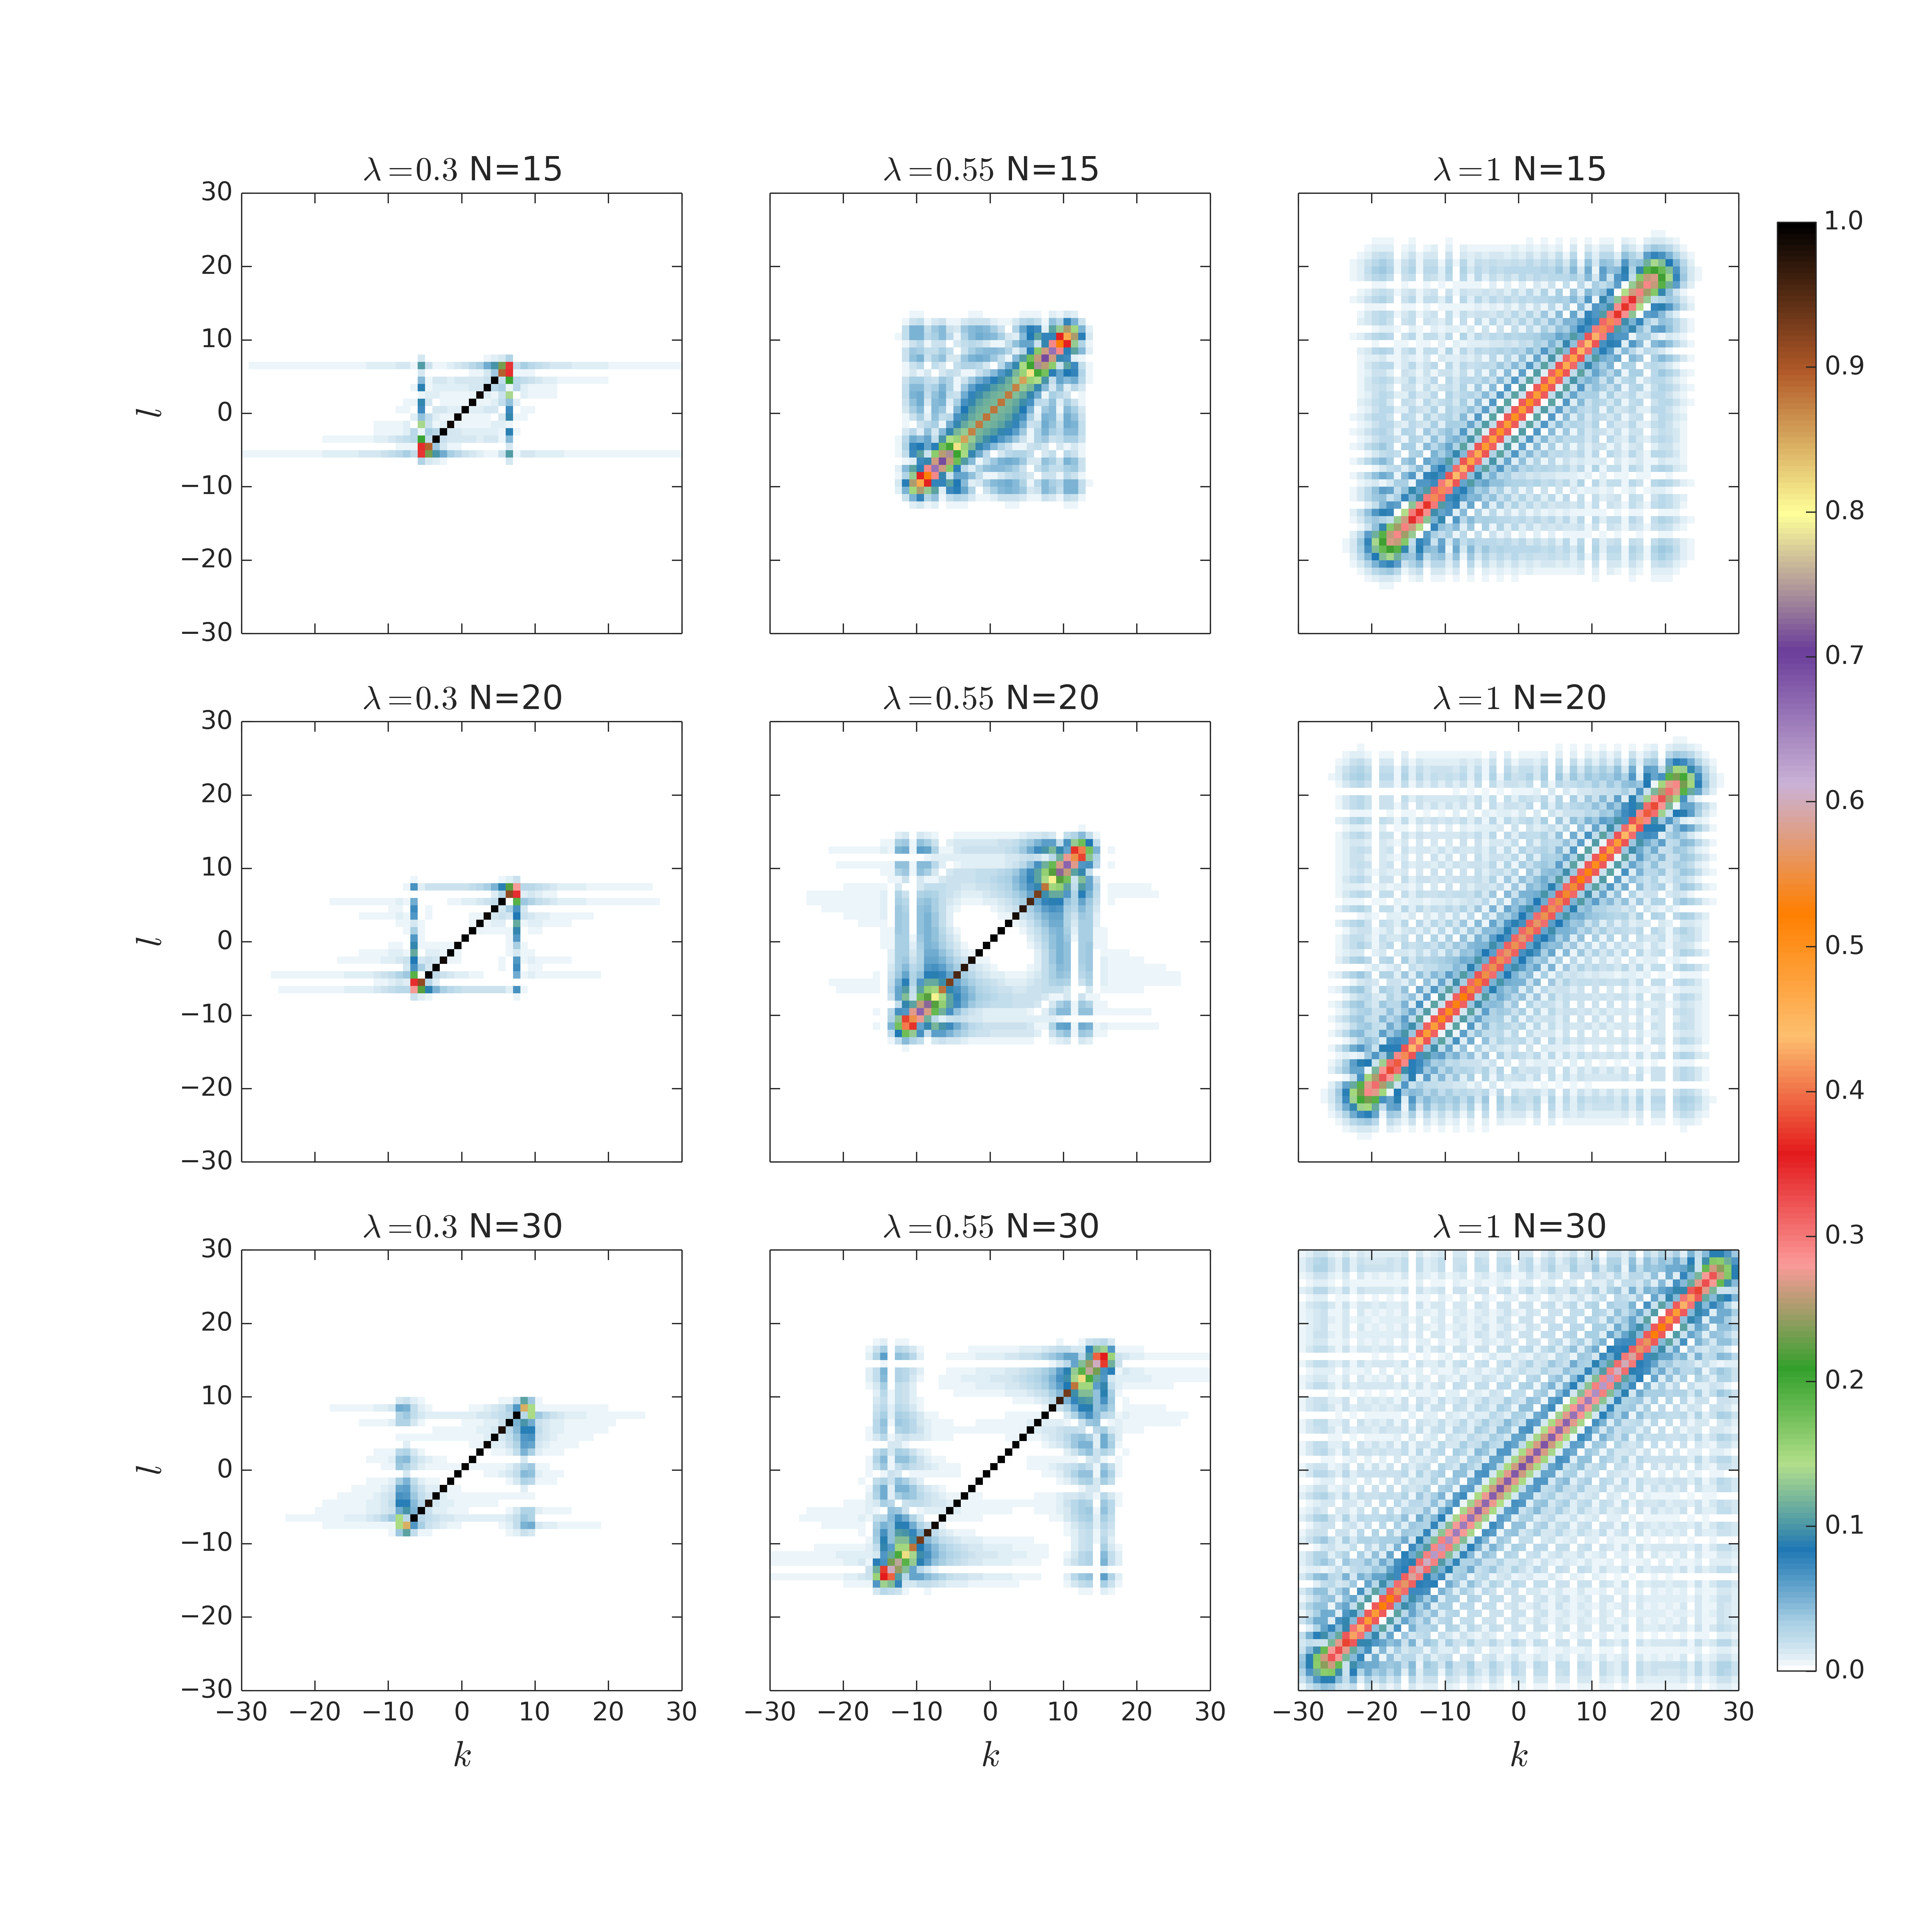
\includegraphics[width=\textwidth]{Hermite/Fig/TmatrixesPlot.png}
\par\end{centering}
\caption[Transfer $T$-matrices]{Nine examples of the absolute values of the transfer $T$-matrices for three different values of $\lambda$ and  three different values of the Hermite decomposition order $N$. 
The number of Fourier coefficients is $M=60$, and the input box size is $L_{box}=23.0$ \AA, which mimics
the first fitting example shown below.
Hermite decomposition orders are $N\in\{15, 20, 30\}$, parameter $\lambda$ takes the values of 0.3 \AA$^{-1}$, 0.55 \AA$^{-1}$, and 1.0 \AA$^{-1}$.
The first column corresponds to the relative $\lambda L_{box}$ value of 6.9, the middle column corresponds to the relative $\lambda L_{box}$ value of $12.65$, and the 
right column to the relative $\lambda L_{box}$ value of $23$.
Notably, at low values of $\lambda$ the transfer matrix encodes only small order reflexes. The index of the last reflex can be estimated  from Eq. \ref{eq:OmegaMax} as $k_{max}=\frac{\sqrt{2N+1}\lambda L_{box}}{2\pi}$.
Increasing the value of $\lambda$, the number of encoded frequencies rises. However, at the same time, the quality of encoding of low frequencies worsens, as can be seen from the values at the diagonal.
}
\end{figure}

\subsection{Asymptotic behaviour of the transfer matrix}
Here we demonstrate that the transfer matrix asymptotically  achieves the  Kronecker delta function at $N\rightarrow\infty$.
%[To gain deeper understanding of the T-matrix behaviour we show the assimptotics of this matrix for $N\rightarrow\infty$.] 
Recall the Mehler's formula \cite{Mehler1866ueber}:
\begin{equation}
\sum_{n=0}^N u^n \psi_n(x)\psi_n(y)=\frac{1}{\sqrt{\pi(1-u^2)}} \exp \left( -\frac{1-u}{1+u}\frac{(x+y)^2}{4} - \frac{1+u}{1-u}\frac{(x-y)^2}{4} \right)
\end{equation}
If we rewrite the transfer matrix in the following way:
\begin{equation}
T_{k,l} = \frac{1}{L_{box}} \int_{-L_{box}/2}^{+L_{box}/2}dx~ \sum_{n=0}^{N}(-i)^n \psi_{n}(\frac{k}{L_{box}}; \frac{2\pi}{\lambda}) e^{2\pi i l x/L_{box}}\psi_{n}(x; \lambda),
\end{equation}
and use the fact that
\begin{equation}
\psi_{n}(x; \lambda) \equiv \sqrt{\lambda}\psi_{n}(\lambda x),
\end{equation}
we see that we can use the Mehler's formula to compute the limit
\begin{equation}
\lim_{N\rightarrow\infty} \sum_{n=0}^{N} (-i)^n \psi_{n}(\frac{k}{L_{box}}; \frac{2\pi}{\lambda})\psi_{n}(\frac{l}{L_{box}}; \lambda)
\end{equation}
%
After a simple derivation, we obtain the final result:
\begin{equation}
\lim_{N\rightarrow\infty}T_{k,l} = \frac{1}{L_{box}} \int_{-L_{box}/2}^{+L_{box}/2} e^{2\pi i l x/L_{box}} e^{-2\pi i k x/L_{box}} dx,
\end{equation}
which is exactly the Kronecker delta function.


\subsection{Encoding quality}
There are several ways to evaluate the quality of a model encoding with the subsequent reconstruction. 
For example, in the optimal control theory \cite{boyd1991linear}, the quality of a linear filter is estimated using a certain norm of the transfer matrix.
However, in crystallography, the most used quality criterion is the crystallographic R-factor \cite{stout1968x}:
\begin{equation}
R = \frac{ \sum_{l}\left|\left|\tilde{F}_{l}^{exact} \right| - \left|\tilde{F}_{l}^{mod} \right| \right|}{\sum_{l}\left|\tilde{F}_{l}^{exact} \right|}
,\label{eq:Rfactor}
\end{equation}
where $F^{exact}$ and $F^{mod}$ are the exact Fourier coefficients of a molecule and the coefficients computed from the Hermite coefficients, respectively.
This quantity is a widely used measure of agreement between a crystallographic model and the corresponding experimental X-ray diffraction data. In the case of an ideal electron density
encoding, R-factor is equal to zero. In protein crystallography, models with R-factors less than 0.2 are regarded as good when working at a middle resolution.

%
Equations for the transfer matrix allow to estimate the R-factor values for certain classes of electron density distributions. 
As described above (Eq. \ref{eq:protein_density}), we use the Gaussian distribution to model the electron density of an atom. 
%
Exact Fourier coefficients of a molecule with $N_{atoms}$ atoms at positions $\mathbf{r}_{i}$ are then given as: 
\begin{equation}
{\tilde f}_{l,m,n}^{exact}({\bf s})= \alpha^3 \pi^\frac{3}{2} \sum_{i=1}^{N_{atoms}} e^{ - \alpha^2 \pi^2 {\bf s}_{lmn}^2  } e^ { -2 i \pi \mathbf{r}_{i} {\bf s}_{lmn} }
,\label{eq:ExactCoef}
\end{equation}
where $s_{l,m,n}$ is the wave vector,  ${\bf s}_{l,m,n}=\left( l/L_x,m/L_y,n/L_z \right)$, with $L_x$, $L_y$,  and $L_z$ the dimensions of the bounding box along the corresponding axes.
Similarly, one-dimensional exact Fourier coefficients of the Gaussian function are given as:
\begin{equation}
{\tilde f}_{l}^{exact} =\alpha \pi^\frac{1}{2} \sum_{i=1}^{N_{atoms}} e^{ - \alpha^2 l^2 / L_{box}^2 } e^ { -2 i \pi {r}_{i} l /  L_{box}}
\label{eq:ExactCoef1D}
\end{equation}
To see how the Hermite basis encodes Gaussian densities with various level of detail, we built models of electron density map with different parameters $\alpha$. The 
width of the Gaussian determines the resolution of the density map according to:
\begin{equation}
R=\frac{\pi\alpha}{2}
\label{eq: densityModelAlphaVsResolution}
\end{equation}
The derivation of this formula follows the one well known in crystallography, which describes the extinction of diffraction reflexes. For the sake of completeness of the thesis, we provide 
its derivation in the section \ref{Sec: ResolutionModel}.

To estimate R-factor for certain model parameters, we assume that the input electron density is given as a sum of Gaussians with variance of $\alpha/\sqrt{2}$ equispaced at a distance $\alpha$.
Figure \ref{fig:RfactorsVsNVsLambda} shows analytical R-factors in one dimension computed using Eqs. \ref{Eq:fourierApproximation} and \ref{eq:ExactCoef1D}
as a function of the Hermite decomposition order $N$ and the scaling parameter $\lambda$.
We bounded the input and output frequencies by $M=30$ Fourier coefficients. The size of the input interval $L_{box}$ is set to 23.0 \AA ~ to mimic
the alpha-conotoxin PnIB peptide (pdb code 1AKG) decomposition used in the fitting example below.

\begin{figure}[h]
\label{fig:RfactorsVsNVsLambda}
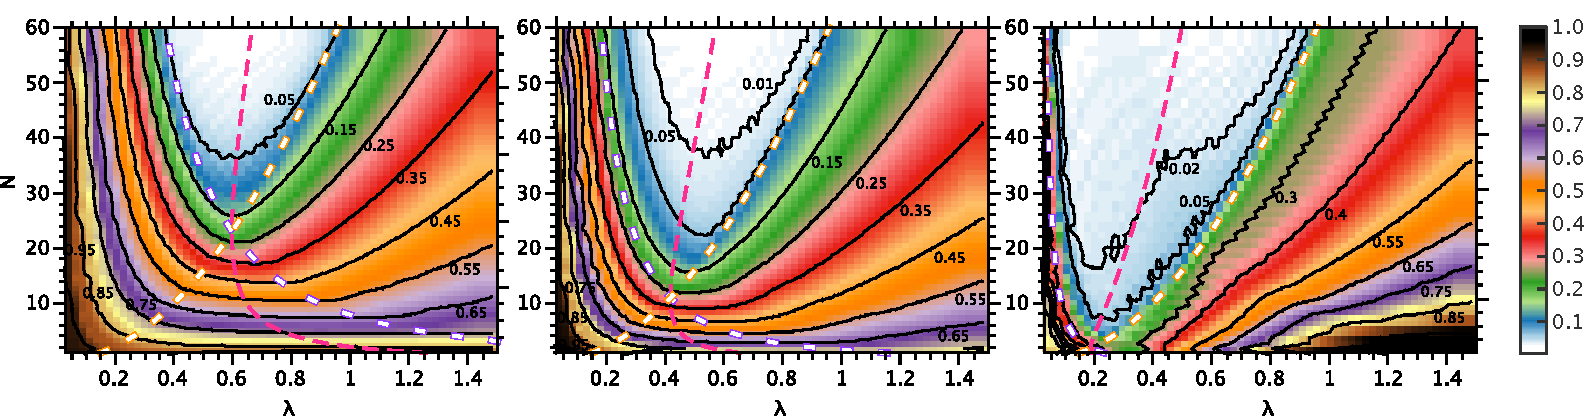
\includegraphics[width=\textwidth]{Hermite/Fig/RfactorsLamN.pdf}
\caption[Analytical R-factors]{
Analytical R-factors in one dimension as a function of Hermite decomposition order $N$ and scaling parameter $\lambda$ computed at three different resolutions.
The input signal is modelled as a sum of Gaussians (Eq. \ref{eq:protein_density}) with the variance of $\alpha/\sqrt{2}$ equispaced at a distance $\alpha$. The number of Fourier coefficients is $M=30$, and the input box size is $L_{box}=23.0$ \AA.  These values are chosen to mimic
the 1AKG peptide decomposition. The estimate on the optimal parameter $\lambda$ (Eq. \ref{eq:LambdaEstimate}) is plotted with the red dashed line. 
The real-space bound on the optimal parameter $\lambda$  (Eq. \ref{eq:encodingRegion}) is shown with the orange dashed line. The reciprocal-space bound on the optimal parameter $\lambda$  (Eq. \ref{eq:levelOfDetails}) is shown with the blue dashed line.
{\bf Left}: The Gaussian parameter $\alpha=0.2$ \AA, corresponding to the absolute input signal resolution of $R=0.31$ \AA~ and the relative resolution of  $R/L_{box}=0.014$. However, in this case, the actual absolute resolution is cut at $L_{box}/M=0.77$ \AA, which corresponds to the relative resolution of 0.033.
{\bf Middle}: The Gaussian parameter $\alpha=1.0$ \AA, corresponding to the absolute input signal resolution of $R=1.57$ \AA~ and the relative resolution of  $R/L_{box}=0.068$.
{\bf Right}: The Gaussian parameter $\alpha=5.0$ \AA, corresponding to the absolute input signal resolution of $R=7.85$ \AA~ and the relative resolution of  $R/L_{box}=0.34$.
}
\end{figure}

%
We should stress that due to the properties of the Hermite functions, 
the whole model is scale--invariant. More precisely, if we keep the product $\lambda L_{box}$ constant, then the relative shape of the Hermite basis functions would not change. Also, if we scale $L_{box}$ and $\alpha$ simultaneously, then the value of R-factor is unchanged. 
%
Therefore, it is useful to provide relative resolutions computed as  $R/L_{box}$.
%
Figure \ref{fig:RfactorsVsNVsLambda} (Left) shows R-factors for the Gaussian parameter $\alpha=0.2$ \AA, corresponding to the absolute input signal resolution of $R=0.31$ \AA~ and the relative resolution of  $R/L_{box}=0.014$. However, in this case, the actual absolute resolution is cut at $L_{box}/M=0.77$ \AA, which corresponds to the relative resolution of 0.033.
%
Figure \ref{fig:RfactorsVsNVsLambda}  (Middle) shows R-factors computed using the Gaussian parameter $\alpha=1.0$ \AA, corresponding to the absolute input signal resolution of $R=1.57$ \AA~ and the relative resolution of  $R/L_{box}=0.068$.
Figure \ref{fig:RfactorsVsNVsLambda} (Right) shows R-factors computed using the Gaussian parameter $\alpha=5.0$ \AA, corresponding to the absolute input signal resolution of $R=7.85$ \AA~ and the relative resolution of  $R/L_{box}=0.34$.
%
The estimate on the optimal parameter $\lambda$ (Eq. \ref{eq:LambdaEstimate}) is plotted with the red dashed line. 
The real-space bound on the optimal parameter $\lambda$  (Eq. \ref{eq:encodingRegion}) is shown with the orange dashed line. The reciprocal-space bound on the optimal parameter $\lambda$  (Eq. \ref{eq:levelOfDetails}) is shown with the blue dashed line.
We see that lowering the resolution of the input signal, R-factors decrease, as can be expected from general considerations. We can also see that the the lower (Eq. \ref{eq:encodingRegion}) and the upper (Eq. \ref{eq:levelOfDetails}) bounds on the optimal scaling parameter $\lambda$ follow the isolines of the R-factor map.
Therefore, their mean given by Eq. \ref{eq:encodingRegion} provides a reasonable estimation on the optimal value of $\lambda$.


Figure \ref{fig:RfactorsVsResolution} shows R-factors as a function of input signal resolution $R$ for three different Hermite decomposition orders $N$, 15, 20, and 30.
R-factors were estimated in the same way as in the previous case. 
More precisely, we assumed the same shape of input electron density and then used Eqs. \ref{Eq:fourierApproximation} and \ref{eq:ExactCoef1D} to compute the analytical R-factors. For these plots, we computed the optimal scaling parameter $\lambda$ using Eq. \ref{eq:encodingRegion}.
Parameter $L_{box}$ and the size of the transfer matrix $M$ were constant and equal to 23 \AA~ and $30$, correspondingly. As in the previous figure, these values are chosen to mimic
the alpha-conotoxin PnIB peptide decomposition used in the fitting example below.
%
The scale of the top horizontal axis gives the absolute resolution for $L_{box}=23$ \AA. The scale of the bottom horizontal axis gives  the relative resolution. In order to compute the absolute resolution, its values need to be multiplied by the chosen value of  $L_{box}$.
As expected, the values of R-factors diminish as the resolution becomes lower. This is because at low resolutions, low-frequency columns of the transfer matrix become more important.
In the limiting cases of zero and infinite resolutions, R-factor can be computed directly from the transfer matrix as a certain norm of $T-I$. For the infinite resolution limit, it is given as $L_1$ norm of the central column of matrix $T-I$. For the zero resolution limit, R-factor is given by the entry-wise $L_1$ norm of $T-I$, $R=\sum_{i,j}|T_{i,j}-\delta_{i,j}|$.
%
Figure 8 also shows an estimation of R-factors for the 3D case. It is based on the assumption that  the Hermite decomposition encoding in 
3D behaves similar to the 1D case, with the number of coefficients scaled as $N_{1D} = \sqrt[3]{N_{3D}}$.

\begin{figure}[H]
\label{fig:RfactorsVsResolution}
\begin{centering}
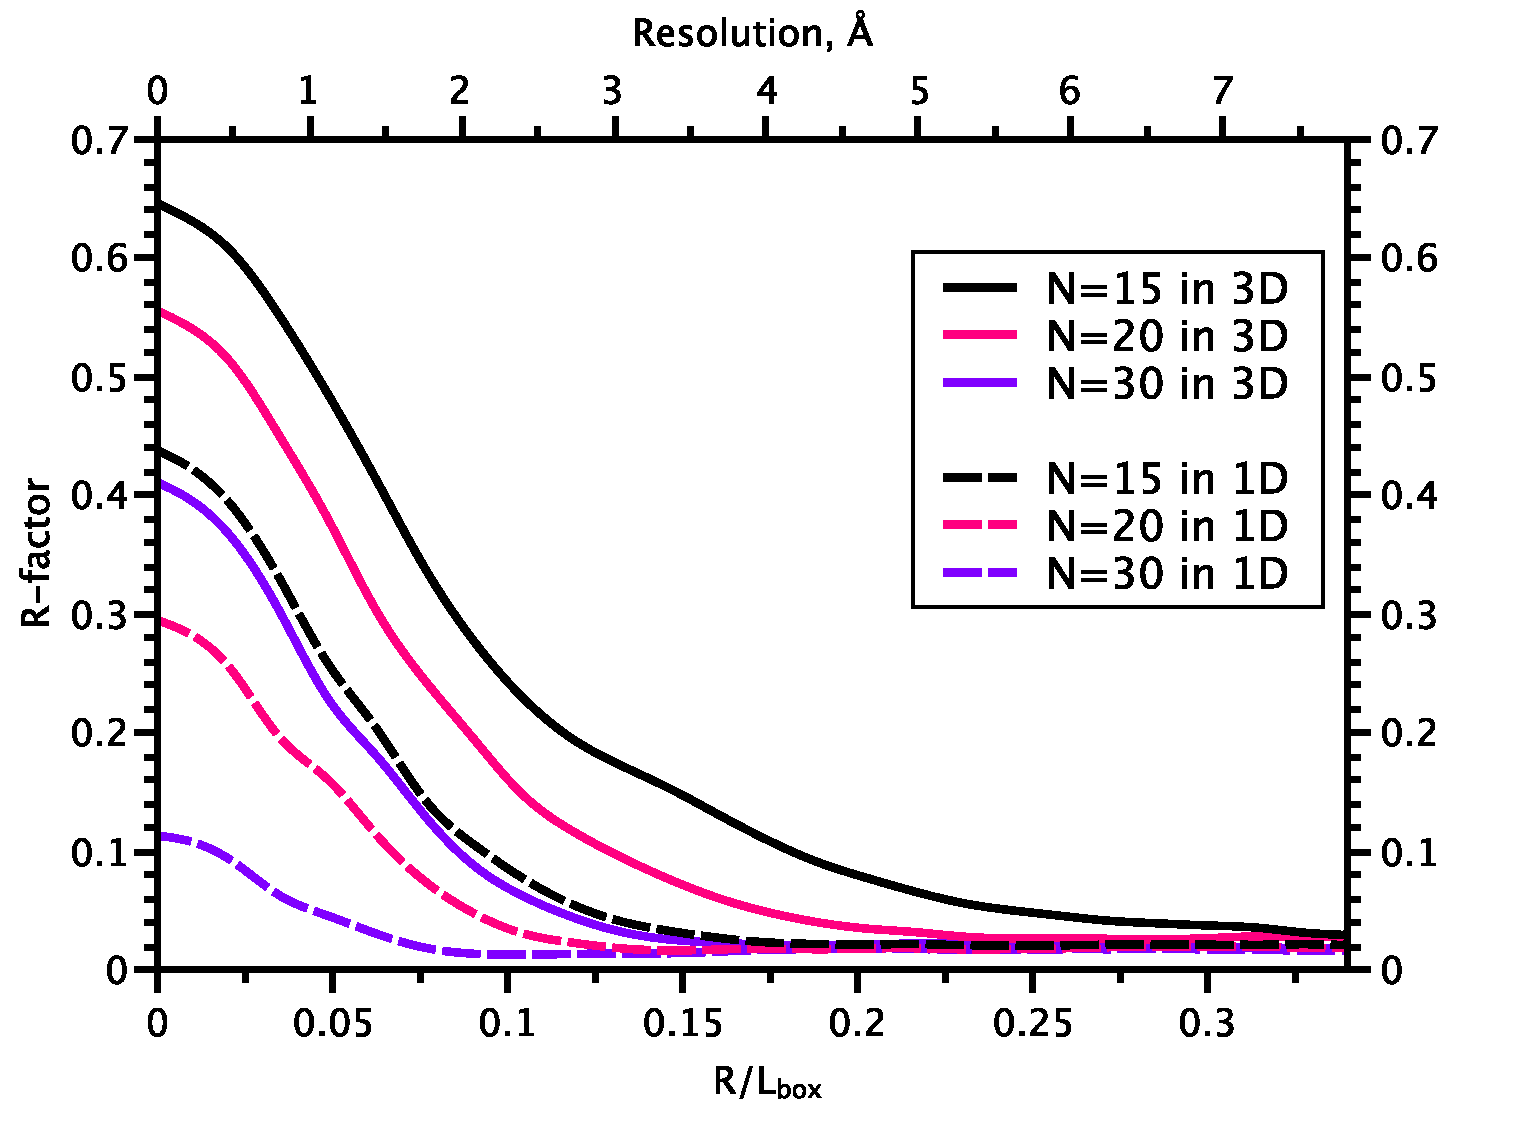
\includegraphics[width=0.5\textwidth]{Hermite/Fig/RfactorVsResolution_DiffAlphas.pdf}
\par\end{centering}
\caption[R-factors in one and three dimensions]{Analytical R-factors in one and three dimensions as a function of  relative resolution $R/L_{box}$. 
The absolute resolution at box size $L_{box}=23$ \AA~ is shown in the top horizontal axis.
Plots for three different Hermite expansions orders are shown, $N\in\{15,20,30\}$.
Parameters $L_{box}$ and $M$ were constant and equal to $23$ \AA~ and $30$, correspondingly. Scaling parameter $\lambda$ was estimated 
using  Eq. \ref{eq:LambdaEstimate}. }
\end{figure}

\subsection{Resolution model}
\label{Sec: ResolutionModel}
To illustrate the connection between parameter $\alpha$ in the model of electron density (Eq. \ref{eq:protein_density}) and the resolution of 
the X-ray diffraction pattern, we use the simplest model. More precisely, we model the electron density as the 
array of Gaussians in a perfect 1D lattice perpendicular to the incoming radiation beam. Parameter $\alpha$ then plays the role similar to the temperature B-factors.
X-ray diffraction intensity depends on the angle between the incoming beam and the direction to the detector $\theta$ as:
\begin{equation}
I \propto \left|\int dx~ f(x)\exp\left( 2\pi i x \frac{\sin\theta}{\lambda}\right)\right|^2
\end{equation}
where $\lambda$ is the wavelength of the incoming radiation. Using the model density (Eq. \ref{eq:protein_density}), we obtain:
\begin{equation}
I \propto \left|\alpha\sqrt{\pi}e^{-(\pi \frac{\sin\theta}{\lambda} \alpha)^{2}} \int dx~ \rho(x)\exp\left( 2\pi i x \frac{\sin\theta}{\lambda}\right)\right|^2
,
\end{equation}
where $\rho(x)$ is the sum of delta functions at the atomic positions. Therefore, the extinction of the diffraction peaks
is proportional to $\left|e^{-(\pi \frac{\sin\theta}{\lambda} \alpha)^{2}}\right|^2$, where we neglect the quadratic factor before the exponent. 
%
According to the definition used in crystallography, resolution is the inter-planar distance in the real space corresponding to the last observable peak in the reciprocal space. 
Unfortunately, the index of the last peak depends on the detector's noise and strongly depends on the characteristics of the measurement device. Therefore, to give qualitative estimation
on the dependence of resolution on the model parameter $\alpha$, we assume that the last observable peak is the one whose intensity decreases approximately by the factor $e^2$. 
The corresponding angle then reads:
\begin{equation}
\sin\theta_{max}=\frac{\lambda}{\pi\alpha}
\end{equation}
Therefore, the minimum inter-planar distance, or, the resolution is given by Bragg's law as:
\begin{equation}
R=\pi\alpha/2 \label{eq:RFactorAppendix}
\end{equation}
